\documentclass[UTF8]{ctexart}[a4paper,10pt]
\usepackage{amsmath}
\usepackage{amsfonts,amssymb} 
\usepackage{thmtools}
\usepackage[hmargin=2.5cm,vmargin=2.5cm]{geometry}
\usepackage{tikz-cd,tikz}
\usepackage{graphicx,float}
\usepackage{fancyhdr}
\usepackage{fourier-orns}
\usepackage[thmmarks]{ntheorem}
\usepackage{quiver}
%声明环境
\newtheorem{example}{例}[section]              
\newtheorem{algorithm}{算法}[subsection]
\newtheorem{theorem}{定理}[section]            
\newtheorem{definition}{定义}[section]
\newtheorem{axiom}{公理}[section]
\newtheorem{property}{性质}[section]
\newtheorem{proposition}{命题}[section]
\newtheorem{lemma}[theorem]{引理}
\newtheorem{corollary}[theorem]{推论}
{
    \theoremheaderfont{\sffamily}
    \newtheorem*{remark}{注解} 
}
\newtheorem{condition}{条件}
\newtheorem{conclusion}{结论}[section]
\newtheorem{assumption}{假设}
{
\theoremstyle{nonumberplain}
\theoremheaderfont{\bfseries}
\theorembodyfont{\normalfont}
\theoremsymbol{\mbox{$\Box$}}
\newtheorem{proof}{证明}
}
%定义命令
\def\N{\mathbb{N}}
\def\Z{\mathbb{Z}}
\def\Q{\mathbb{Q}}
\def\R{\mathbb{R}}
\def\C{\mathbb{C}}
\def\S{\mathbb{S}}
\def\D{\mathbb{D}}
\def\H{\mathbb{H}}
\def\B{\mathcal{B}}
\def\O{\mathcal{O}}
%外测度
\def\outmQ{m_*(Q)}

%页眉设计
\renewcommand 
\headrule{
\hrulefill
\raisebox{-2.1pt}
{\quad{\FourierOrns M T S N}\quad}
\hrulefill}
\pagestyle{fancy}

%超链接红色
\usepackage[colorlinks,linkcolor=red]{hyperref}

\usepackage{enumerate}


\title{General Topology Stduy Notes}
\author{颜成子游}
\begin{document}
    \maketitle
    \newpage
    \tableofcontents
    \newpage
    \section{集合论与逻辑}
    本章聚焦于初步的集合理论和一些逻辑。由于总体来说不是很难,因此笔记会写的比较粗略。
    \subsection{集合的基础概念}
    这一小节主要是给出了集合的若干基础概念的精确定义。\\
    \textbf{属于,不属于,等于,子集,真子集,包含,真包含,并,交,补}

    Tips:

    1.\textbf{“无意义的正确”}指条件就错误的命题。如:“若$x^2<0$,那么颜成子游就能找到女朋友。”这样的话是正确的,但是这句话毫无意义。因为本身
    $x^2<0$就不可能成立。(可以观察它的逆否命题)

    2.\textbf{补}的概念用于多种情况。
    $$
    A-B=\{x|x \in A \quad \text{and}\quad  x \notin B  \}
    $$
    被称为B关于A的补。即不需要$B \subset A$。

    3.集合的若干规则:
    \begin{enumerate}[{(i)}]
        \item 集合“分配律” $A\cap(B \cup C)=(A\cap B)\cup (A\cap C)$
        \item  $A\cup(B \cap C)=(A\cup B)\cap (A\cup C)$
        \item 德摩根定理: $A-(B \cup C)=(A-B)\cup(A-C)$
        \item $A-(B \cap C)=(A-B)\cup (A-C)$
    \end{enumerate}

    4.\textbf{集簇}。

    5.任意闭和任意交:需要注意的是,如果集簇本身是一个空集,即:
    $$
    \bigcup_{A \in \mathcal{A}}A=\{x|x \in A\quad \text{for at least one} A \in \mathcal{A}\}
    $$
    和
    $$
    \bigcap_{A \in \mathcal{A}}A=\{x|x \in A\quad \text{for everyone} A \in \mathcal{A}\}
    $$
    我们观察定义,可以发现,对于第一个式子,可以看出没有$x$满足;对于第二个式字,所有$x$都“无意义”地满足。因此:
    $$
    \bigcup_{A \in \mathcal{A}}A=\emptyset \bigcap_{A \in \mathcal{A}}=X
    $$
    \subsection{函数}
    我们将使用笛卡尔积来表示函数。

    \begin{definition}[指派法则]
        指派法则是两个集合的笛卡尔积$C\times D$的一个子集$r$,该子集满足这样的条件:$C$的每一个元素最多是$r$中的一个有序偶对的第一个坐标。

        像集=$\{d|存在c\in C ,使得(c,d)\in r\}$.

        定义域=$\{c|存在d \in D,使得(c,d)\in r\}$
    \end{definition}
    若$(c,d)$和$(c,d^{*})$都属于$r$,那么$d=d^*$。
    
    \textbf{值,像,限制,复合,单,满,一一的,原像}等概念不再赘述。

    下面有一个常用的引理判断单满射(不从定义出发,范畴式的)
    \begin{lemma}
        设$f:A \to B$,如果存在函数$g:B \to A$满足对于$f\circ g:B \to B$,$f\circ g(x)=x ,\forall x \in B$。则$f$是一个满射。

        若存在函数$h:B\to A$满足对于$h\circ f:A \to A$,$h\circ f(x)=x,\forall x \in A$,则$f$是单射。
    \end{lemma}
    如果$g$和$h$是同一个函数(事实上,如果他们都存在,那么就是),称其为$f$的逆函数(反函数)。
    \subsection{关系}
    关系是比函数更宽泛的概念。它只是集合笛卡尔积的子集:
    \begin{definition}
        集合A上的一个关系是笛卡尔积$A\times A$的一个子集$C$。

        $x,y$有关系$C$记作$xCy$。
    \end{definition}
    \textbf{等价关系}的定义不再赘述。但要注意,什么时候平行才不是等价关系。

    等价关系的记号:$\thicksim$。

    给定集合$A$的一个等价关系$\thicksim$,和$A$的一个元素$x$,可以得到:
    $$
    E=\{y:y\thicksim x\}
    $$
    为$x$的等价类。

    显然,一个集合的所有等价类要么相同,要么不交。我们把集合$A$的所有不交的等价类形成的集簇记为$\mathcal{E}$

    下面的定义描述对集合进行拆分,其本质就是一个等价关系(显然的):
    \begin{definition}
        集合$A$的一个分拆是$A$的无交子集的一个族,其并为$A$.
    \end{definition}
    
    \textbf{序关系}又称全序关系或者线序关系。
    \begin{definition}
        集合$A$中的一个关系$C$被称为\textbf{序关系},如果其满足:
    \begin{enumerate}[(a)]
        \item $\forall x, y \in A,x\neq y$,则有$xAy$或$yAx$。
        \item $A$中没有$x$,使得$xCx$成立。
        \item 若$xCy$,$yCz$,则$xCz$也成立。
    \end{enumerate}
    \end{definition}
    即可比较性,不自反性,传递性。常用$<$来表示序关系。
    \begin{definition}
        如果$X$是一个集合,$<$是定义在上面的一个全序关系,那么集合$E$:
        $$
        E=\{x:a<x<b\}
        $$
        是一个开区间。如果其是空集,那么$a$为$b$紧接前元,$b$为$a$的紧接后元
    \end{definition}
    \begin{definition}
        称分别含有序关系$<_A,<_B$的集合$A$和$B$的序型相同,如果在它们之间有一个一一的保序映射$f:A\to B$,使得
        $$
        a_1<_A a_2 \Rightarrow f(a_1)<_B f(a_2)
        $$
        
    \end{definition}
    对于保序映射而言,当然把紧接前元和紧接后元映射为紧接前元和紧接后元。

    有些时候我们想要构造全序关系。下面给出一个常用的方式:
    \begin{definition}[字典序关系]
        分别含有序关系$<_A,<_B$的集合$A$和$B$的笛卡尔积$A \times B$可以定义这样的全序关系:
       
        当 $a_1<_A a_2$或者当$a_1=a_2$并且$b_1<_B b_2$时,
        $$
        a_1 \times b_1 <a_2 \times b_2
        $$
    \end{definition}
    字典序的名字来源于英文字典对单词的排序方式。
    
    接下来们讨论“界”的概念。
    \subsubsection*{界(确界)}
    相对于通常的大于小于关系,我们也可以类似的给出序关系中的\textbf{最小元,最大元,上界,上确界,下界,下确界,上(下)确界性质}的概念。
    当然,这里使用的定义都是最trival的。

    下面给出上确界性质和下确界性质。并给出他们是等价的证明。
    \begin{definition}
        如果全序集合$A$的每一个非空有上界的子集$A_0$都必有上确界,则称$A$具有\textbf{上确界性质}。
        同样,如果全序集合$A$的每一个非空有下界的子集$A_0$都必有下确界,则称$A$具有\textbf{下确界性质}。
    \end{definition}
    \begin{theorem}
        $A$具有上确界性质,当且仅当其有下确界性质。
    \end{theorem}
    \begin{proof}
        设$A$有上确界性质。现在给定一个子集$A_0$,其有下界。我们证明其下界集$B$一定有最大值。

        $B$显然有上界($A_0$的任何一个元素都是)。因此根据上确界性质,其有上确界$b$。我们证明$b \in B$。

        如果$b \notin B$,那么$b$不是$A_0$的下界。即存在$a \in A_0$,$a_0<b$。

        但是$a_0$也是$B$的一个上界,因此根据$b$是上确界得:$b \leq a_0$。这产生了矛盾!故$b \in B$,即下界集有最大值。

        同理也可从下确界性质推导上确界性质。

    \end{proof}
    \begin{example}
        集合$(0,1)$拥有上确界性质。因为任何一个有上界的集合都有上确界(有上界意味着另一边不能是“1)”)。集合$[0,1)$也拥有。
    \end{example}
    \begin{example}
        在字典序下的$[0,1]\times[0,1]$具有上确界吗?对于$[0,1]\times [0,1)$呢?对于$[0,1)\times [0,1]$呢?
    \end{example}
    \subsection{整数与实数}
    实数是什么?这里,我们把实数看作是一个具有若干条公理的集合。其必然的结果就是实数。其次,我们从实数的角度出发,给出整数的定义。
    尽管这似乎与数字的发展历程完全相反,但在逻辑上更加自洽。

    回忆:\textbf{二元运算}是一个将$A \times A$映射到$A$的函数。

    \begin{definition}
        一个集合$\R$被称为实数,若其存在两个运算“加法”和“乘法”,以及一个全序关系“$<$”,并存在以下若干性质:
        \begin{enumerate}[{(1)}]
            \item $(x+y)+z=x+(y+z),(xy)z=x(yz)$
            \item $x+y=y+x,xy=yx$
            \item 有零元
            \item 有幺元
            \item 除0外每个元素都有逆元,所有元素都有负元
            \item $x(y+z)=xy+xz$
            \item 若$x>y$,则$x+z>y+z$。
            \item 若$x>y,z>0$,则$xz>yz$。
            \item 全序关系具有上确界性质
            \item 对于任何的$x<y$,都有$z$,使得$x<z<y$。
        \end{enumerate}
    \end{definition}
    删去实数的一些性质,就得到了一些弱化的结构:
    
    1.满足前六条的代数结构称为\textbf{域}。\\
    2.满足7,8性质的域称为\textbf{有序域}。\\
    3.满足最后两条的集合称为\textbf{线性连续统}\\
    
    接下来讨论整数:
    \begin{definition}
        实数集的一个子集$A$称为归纳的,如果它包含数1,并且只要$x \in A$,则必有$x+1 \in A$。设$\mathcal{A}$为$\R$中所有包含1的归纳子集的族。
        正整数$\Z_+$定义为:
        $$
        Z_+=\bigcap_{A \in \mathcal{A}}A
        $$
    \end{definition}
    一个集合如果只含有正整数,并且归纳,那么其就是正整数。

    整数集合定义为正整数,0,以及所有正整数的负元所构成的集合。

    定义:$S_{n+1}$代表集合$\{1,2,3,4,5\dots ,n \}$

    还有两个引理:良序定理和第二数学归纳法。良序定理将在之后阐述。第二数学归纳法是显然的。不再讨论。
    \subsection{笛卡尔积}
    广义的笛卡尔积是我们着重探讨的对象。
    \begin{definition}
        设$\mathcal{A}$是一个非空集簇,$\mathcal{A}$的指标函数是从某一个集合$J$到$\mathcal{A}$的一个满射$f$,其中$J$称为指标集。族$\mathcal{A}$
        连同指标函数$f$一起称为一个集的加标族或加标集簇。给定$a\in J$,集合$f(a)$记为$A_a$。这个加标集簇本身记为:
        $$
        \{A_\alpha\}_{\alpha \in J}
        $$
    \end{definition}

    指标集可以帮助我们更简单的描述集簇的一些操作。

    \begin{definition}
        设$m$是一个正整数;对于给定的集合$X$,$X$中的元素的一个\textbf{$m$-串}定义为函数:
        $$
        x: \{1,2,3,\dots,m\} \longrightarrow X
        $$ 
        函数本身用$(x_1,x_2,x_3,\cdots.x_m)$来表示序关系。
        
        现在设$\{A_1,A_2,A_3,\dots,A_m\}$是一个以$\{1,2,3,\dots,m\}$为指标集的加标集簇。令$X=\bigcup_{i=1}^m A_i$,那么这个集簇的笛卡尔积记作:
        $$
        \prod_{i=1}^m A_i 
        $$
        定义为$X$中所有$m$串的子集,使得对于每个$i$有$x_i \in A_i$
    \end{definition}
    
    显然,多个集合的笛卡尔积与一个集合一个集合的笛卡尔积没有太大的区别。他们存在十分简单的一一对应。因此我们不讨论其区别,认为两种方式的定义都是合理的。

    下面给出可数个集合的笛卡尔积。它与有限的情况在性质方面会有不少不同。

    \begin{definition}
        对于给定的集合$X$,$X$中的元素的一个\textbf{$\omega$-串}定义为函数:
        $$
        x: \Z^+\longrightarrow X
        $$ 
        函数本身用$(x_1,x_2,x_3,\cdots)$来表示。
        
        现在设$\{A_1,A_2,A_3,\dots\}$是一个以$\{1,2,3,\dots\}$为指标集的加标集簇。令$X=\bigcup_{i=1}^\infty A_i$,那么这个集簇的笛卡尔积记作:
        $$
        \prod_{i=1}^\infty A_i 
        $$
        定义为$X$中所有$\omega$串的子集,使得对于每个$i$有$x_i \in A_i$
    \end{definition}
    接下来的若干节我们将会讨论这两个笛卡尔积的性质。
    \subsection{有限集}
    有限集有一些直观的性质值得我提出来:
    \begin{lemma}
        设$A$是一个集合。假定对于某一个$n\in \Z_+$,存在一个一一对应$f:A \to \{1,\cdots,n\}$。设$B$为A的一个真子集,则不存在一个
        一一对应$g:B \to \{1,\cdots,n\}$。但是(假定其非空),必定存在一个一一对应$h:B \to \{1,\cdots,m\}$对于一个$m<n$成立。
    \end{lemma}
    定理是显然的。使用归纳法也可以从逻辑上严格的证明~。
    
    由此得到的推论更加常用:
    \begin{corollary}
        如果$A$是一个有限集,那么不存在$A$与其真子集的一一对应。
    \end{corollary}
    \begin{corollary}
        设$B$是一个非空集,则下列条件等价:
        \begin{enumerate}[(1)]
            \item $B$是有限集合。
            \item 存在从正整数的某一个截到$B$上的满射。
            \item 存在$B$到正整数的某一个截的单射。
        \end{enumerate}
    \end{corollary}
    \begin{corollary}
        若干个有限集的有限并和有限笛卡尔积是有限集。
    \end{corollary}
    \subsection{可数集和不可数集}
    在有限后,我们就要着手研究无穷的情况。与朴素的想法不同,无穷也是分种类的:
    \begin{definition}
        一个无限集是可数无限的,如果存在一个一一映射对应:
        $$
        f:A \longrightarrow Z_+
        $$
        一个集合如果有限或者可数,那么称它是一个至多可数的集合。
    \end{definition}
    我们将在之后介绍不可数的集合的例子。可数的好处在于它和有限集的性质相似度跟高。在这里,我们先给出至多可数的集合的例子。
    
    \begin{example}
        笛卡尔积$Z_+\times Z_+$是一个可数无限集。想要给出相关的映射,我们就可以从这张图入手:
        \begin{figure}[H]
            \centering
            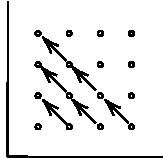
\includegraphics[scale=1.2]{Countable union.pdf}
        \end{figure}
    \end{example}
    这张图本身就描述了一个对应。但具体的映射还是略显困难。我们在后面将说明其严格的证明。

    下面的定理给出了判断一个集合是否为至多可数集合的办法。
    \begin{theorem}
        设$B$是非空的集合,那么下列的条件是等价的:
        
        (1)$B$是至多可数集合。

        (2)存在满射$f:Z_+ \to B$

        (3)存在单射$g:B \to Z_+$
    \end{theorem}
    
    为了配合证明,我们给出一个引理:
    \begin{lemma}
        如果$C$是$\Z_+$的一个无限子集,那么它是可数集。
    \end{lemma}
    \begin{proof}
        我们将构造一个一一对应的$h:\Z_+ \to C$。采用归纳法.定义$h(1)$为$C$中的最小元(根据良序定理)。现在假设$h(1),h(2),\dots,h(n-1)$
        都已经有定义,那么定义$h(n)$为:
        $$
        h(n)=min[C-h(\{1,2,3,\dots,n-1\})]
        $$
        $h(n)$的定义是良定的。因为$C-h(\{1,2,3,\dots,n-1\})$不可能是一个空集,否则就是有限集合。
        容易证明$h(n)$是单射。又因为$C$是无限的。任何一个数总轮的上。因此是满射。从而使一一对应。
    \end{proof}
    注意到这里我们使用了所谓”归纳定义原理”。这个原理来源于归纳法。但由于其细节并非逻辑上的难事,我们不在此论述。

    有了引理,证明定理并不困难。省略。

    \begin{corollary}
        至多可数集的子集是至多可数的。
    \end{corollary}
    \begin{corollary}
        集合$Z_+\times Z_+$是可数无限的。
    \end{corollary}
    \begin{proof}
        给定单射$f: Z_+\times Z_+ \to Z_+$.定义其为:
        $$
        f(n,m)=2^n3^m
        $$
        这是一个单射。因此根据上述定理,可得:集合$Z_+\times Z_+$是可数无限的。
    \end{proof}
    \begin{theorem}
        可数集的可数并也是可数的。可数集的有限笛卡尔积也是可数的。
    \end{theorem}
    \begin{proof}
        设$\{A_n\}$为可数集的一个加标族,其指标集$J$为$\{1,\cdots,n\}$或$\Z_+$。假定所有集合非空。

        因为每个集合$A_n$是可数的,故对于每一个$n$都可以取一个满射$f_n:Z_+ \to A_n$,类似,也有满射$g:Z_+ \to J$。用:
        $$
        h(k,m)=f_{g(k)}(m)
        $$
        定义函数:
        $$
        h:Z_+\times Z_+ \longrightarrow \bigcup_{n \in J}A_n
        $$
        容易验证$h$是一个满射。又$Z_+\times Z_+$是可数集,因此$\bigcup_{n \in J}A_n$也是可数集。

        另一方面,由于两个可数集合的笛卡尔积与$\Z_+\times \Z_+$有着一一对应。因此可数。归纳法得有限个都是成立的。
    \end{proof}
    
    但可数集合的可数笛卡尔积就不一定是可数的。
    \begin{example}
        集合$X=\{0,1\}$。那么$X^\omega$不是至多可数集合。
    \end{example}
    例子的证明我不去讲。希望自己回忆。

    下面这个例子则显得更深刻:
    \begin{example}
        设$A$是一个集合。则不存在单射$f:\mathcal{P}(A) \to A$,也不存在满射$g:A \to \mathcal{P}(A)$
    \end{example}
    \begin{proof}
        一般说来,上述两个集合相伴相生。因此我们只考虑$g:A \to \mathcal{P}(A)$的情况。

        对于任何给定$g:A \to \mathcal{P}(A)$,记:
        $$
        B=\{a|a \in A-g(a)\}
        $$
        即$B$是那些使本身不属于其对应子集的元素的集合。那么$B \subset A$。设$g(b)=B$,若$b \in B$,则与$B$的定义矛盾。若$b \notin B$,那么
        $b$就不属于其对应子集,即$b \in B$。从而导出矛盾!
    \end{proof}
    这个定理的证明非常巧妙。值得思考。
    \subsection{无限集合与选择公理}
    略~
    \subsection{良序集}
    \begin{definition}
        具有全序关系$<$的一个集合$A$称为良序的,如果$A$的任意非空子集有一个最小元。
    \end{definition}
    我们给一些例子来说明良序性:
    \begin{example}
        在字典序下考虑$\{1,2\}\times \Z_+$。它可以表示成一个无穷序列紧跟着另一个无穷序列:
        $$
        a_1,a_2,a_3\dots,b_1,b_2,b_3,\dots,
        $$
        其中每一个元素都比它右边的小。设集合$C$是$\{1,2\}\times \Z_+$的子集:如果$C$包含任何一个$a$,则最小元就是$C$与序列$a_1,a_2,a_3.\dots$的交
        的最小元;如果不含,则$C$是$b_1,b_2,b_3\dots$的一个子集,含有最小元。
    \end{example}
    \begin{example}
        在字典序下考虑$\Z_+\times \Z_+$。对于任何一个给定的子集$C$,我们这样给定其最小元:
        $$
        \text{Define} C_1=\{a|(a,b)\in C\}
        $$
        $C_1$是$\Z_+$的一个子集,因此有最小值$a_0$.取:
        $$
        C_2=\{b|(a_0,b)\in X\}
        $$
        从而$C_2$也是一个$\Z_+$的子集。因此有最小值$b_0$。
        可以验证,$(a_0,b_0)$就是最小值
    \end{example}
    我们有:
    \begin{lemma}
        如果$A,B$都是良序集,那么$A \times B$在字典序下也是良序集。
    \end{lemma}

    下面几条定理是非常重要的:
    \begin{theorem}
        任何一个非空有限全序集具有$\Z_+$的一个截的序型,因而必定是良序集。
    \end{theorem}
    \begin{theorem}[良序定理]\label{well_ordering}
        若$A$是一个集合,则存在$A$上的一个全序关系,使其成为一个良序集。
    \end{theorem}
    良序定理告诉我们,不管集合如何,都能找到一个序关系,使得其称为良序集。这看起来十分不平凡,但是整个证明过程中,最值得商榷
    的地方是选择公理。如果我们承认选择公理,那么就必须承认良序定理。听起来很不错!证明过程在这里给出一个链接:
    \url{https://www.zhihu.com/question/27427705}

    在实际的应用中我们更多使用下面这个比较弱的推论:
    \begin{corollary}\label{thm:well_ordering-}
        存在一个不可数的良序集。
    \end{corollary}
    
    用这个较弱的推论,我们给出一个很有用的良序集:
    \begin{definition}
        设$X$是一个全序集。给定$a \in X$,用$S_a$表示集合:
        $$
        S_a=\{x|x \in X ,x<a\}
        $$
        称为$X$在$\alpha$处的\textbf{截}。
    \end{definition}

    \begin{lemma}
        存在一个以$\Omega$为最大元的不可数良序集$A$,$A$在$\Omega$处的截$\Omega$是一个不可数集,而$A$的其他每一个截都是可数集。
    \end{lemma}
    \begin{proof}
        由推论\ref{thm:well_ordering-}得到了一个不可数的集$A^*$。我们构造:$C=\{1,2\} \times A^*$.记新的集合$A$:
        $$
        A=\{a|S_a \subset C ,\text{is uncountable}\}
        $$
        首先$A$是非空的。因为任何$S_{(2,b)}$就是不可数的。其次由于$C$由$A^*$产生,因此也有良序性质。因此$A$有最小值$\Omega$

        取$S_\Omega$,就得到了我们的不可数良序集。
    \end{proof}\
    这一个集合具有很好的特点:它本身是不可数的,但是它的每个截都是可数的。也就是说它是在序的意义下最小的不可数集合(再小就变成了可数集合)。
    值得指出的是,这样的集合的序型是确定的。也就是说,只考虑序型,我们可以给出这样的集合的一个名字:\textbf{极小不可数良序集}。
    \begin{proof}
        设两个集合$A,A^*$的最大值分别为:$\Omega.\Omega^*$。定义映射:
        $$
        f:A \to A^*
        $$
        
        将$\Omega$的像记为:$\Omega^*$。
    \end{proof}
    
    从极小不可数良序集的构造我们的得知,其任何一个有上界的子集都是可数的。相反,我们也有如下定理:
    \begin{theorem}
        设$A_0$是$S_\Omega$的可数子集,那么$A_0$有上界。
    \end{theorem}
    
    虽然$\Omega \notin S_\Omega$,但是我们仍然说明其有一个上界。这表明在$S_\Omega$中,有上界和可数是等价的。
    \begin{proof}
        设$a \in A_0$,则$S_a$是可数的。又$A_0$是一个可数集,因此,集合
        $$
        S=\bigcup_{a \in A_0} S_a
        $$
        也是可数集合。因此$S \neq S_\Omega$。由此,取$x \notin S$,则$x$是$S$的上界,同时也是$A_0$的上界。

        因此$A_0$有上界。
    \end{proof}
    \section{拓扑空间}
    \subsection{拓扑空间的基本概念}
    点集拓扑学是整个拓扑学的语言。作为语言,其抽象
    \subsection{拓扑基}
    \subsubsection{拓扑基}
    \begin{theorem}[拓扑基公理]
        设$X$是集合,$B \subset P(X)$。若$B$满足:
        \begin{enumerate}[(B1)]
            \item $\bigcup B= X$。
            \item 任给$B_1,B_2 \in B$,及$x \in B_1 \cap B_2$,都存在$B_3 \in B$使$x \in B_3 \subset B_1 \cap B_2$。
        \end{enumerate}
        则存在X上的唯一拓扑$\mathcal{O}$使$\mathcal{B}$是$\mathcal{O}$的基.
    \end{theorem}
    \begin{example}\label{ex:Sorgenfreyline}
        Sorgenfrey直线:
        取$\R$上的拓扑基为:
        $$
        \B=\{ [a,b)|a<b \in \R\}
        $$
        容易验证$\B$满足拓扑基公理,因此构成Sorgenfrey直线的基。
        
        (1)注意到$(a,b)=\bigcup_{n \geq 1}[a+\frac{1}{n}(b-a),b)$,从而Sorgenfrey拓扑比欧氏拓扑强。

        (2)Sorgenfrey拓扑基是闭集。
        
        任取一个集合$[a,b)$,其补为$(-\infty,a)\cup [b,+\infty)$,从而:
        $$
        (-\infty,a)\cup [b,+\infty)=\bigcup_{-n<a}[-n,a) \cup \bigcup_{n>b}[b,n)
        $$
        这表明其补集也是一个开集,从而拓扑基即开且闭。(这比欧氏空间中的要强一些)

    \end{example}
    \begin{example}
        Sorgenfrey平面:取$\R^2$上的拓扑基:
        $$
        \B=\{ [a,b)\times [c,d)|a<b \in \R,c<d \in \R \}
        $$
        与例\ref{ex:Sorgenfreyline}有着相似对应的结果。
    \end{example}
    \begin{example}
        现在我们列举我们知道的$\R$的拓扑:
        \begin{enumerate}
            \item 欧氏拓扑
            \item Sorgenfreytuopu
            \item 离散拓扑
            \item 左拓扑右拓扑
            \item 平庸拓扑
            \item 有限补拓扑
            \item 可数补拓扑
        \end{enumerate}
        推广在平面上,我们可以得到64个拓扑(笑),但一般不会搞这么恐怖(笑)。
    \end{example}
    \begin{example}
        如果存在两个互素的正整数$a,b$,$\gcd(a,b)=1$。令:
        $$
        D_{a,b}=\N \cap\{ak+b|k \in \Z\}
        $$
        例如:$D_{2,3}$是所有的奇数。

        则$D_{a,b}$作为一个基生成了一个Topology。
    \end{example}
    \subsubsection{子基,领域基}
     接下来我们引入子基的概念。子基并不一定可以作为一组基生成拓扑,但是进行“切割”后就可以成为一组基。
     \begin{definition}
         称$\B$是$X$的子基,如果:
         $$
         {X}\cap \{U_1\cap U_2\cap\dots U_n|U_1,U_2,\dots,U_n \in \B\}
         $$
         是$X$的一组基。
     \end{definition}
     \begin{example}
         考虑$\R$上的欧氏拓扑有子基:
         $$
         \{(-\infty,a),(a,+\infty)|a\in \R\}
         $$
         原因是很容易交出开区间。
     \end{example}
     \begin{theorem}[子基定理]
         设$X$是一个集合。任给$X$的子集族,都存在$X$上的唯一拓扑$\mathcal{O}$使得$\B$是$\mathcal{O}$的子基。
     \end{theorem}
     \begin{proof}
         定义$\mathcal{O}$:
         $$
         U \in \mathcal{O} \Leftrightarrow \forall x \in U,\exists B_1,\dots,B_n \in \B, x \in B_1 \cap\dots B_n \subset U
         $$
         接下来的验证是程序性的,不需要再阐明。
     \end{proof}
     \begin{proposition}
         设$(X,\mathcal{O})$是拓扑空间,$Y \subset X$,$\mathcal{B} \subset \mathcal{O}$。则:
         \begin{enumerate}
             \item 若$\B$是$X$的基,则$\{U \cap Y|U \in \b$是$Y$的基。
             \item 若$\B$是$X$的子基,则$\{U \cap Y|U \in \b$是$Y$的子基。
         \end{enumerate} 
     \end{proposition}
     \begin{proof}
         只证明第一个。

         任取$Y$中的开集$V=U \cap Y$,$U$是X的开集。
         $$
         V=U\cap Y=\bigcup \{B \in \B|B\subset U\}\cap Y=\bigcup\{B\cap Y|B \in \B,B \subset U\}
         $$
        \end{proof}
        \begin{proposition}
            设$X,Y$是拓扑空间,$f:X \to Y$,$\B$是$Y$的基,$\B_0$是$Y$的子基。则以下条件等价:
            \begin{enumerate}
                \item $f$连续
                \item $\forall U \in \B$,$f^{-1}(U)$是$X$上的开集。
                \item $\forall U \in \B_0$,$f^{-1}(U)$是$X$上的开集。
            \end{enumerate}
        \end{proposition}
        \begin{proof}
            只证明(2)推导(1):

            任意$Y$中的开集$A$,A分解为基的并,而原像运算时保并的运算的,从而得证。
        \end{proof}
        接下来我们讨论领域基的概念。
        \begin{definition}
            设$X$是拓扑空间,$x \in X$,$\mathcal{A}$是$x$的一族领域(未必是开集)。

            称$\mathcal{A}$是$x$的领域基,若任给$x$的领域$V$都存在$A \in \mathcal{A}$使得:$x \in A \subset  V$。
        \end{definition}
        \begin{example}
            在$\R$的欧氏拓扑下,对于$x$的领域,集合
            $$
            \mathcal{A}=\{(x-1/n,x+1/n)|n \geq 1\}
            $$
            是一个$x$的领域基。

            在Sorgenfrey拓扑下,
            $$
            \mathcal{A}=\{[x,x+1/n)|n \geq 1\}
            $$
            是一个$x$的领域基。

            在度量空间中,对于$x \in X$,
            $$
            \mathcal{A}=\{B(x,1/n)|n \geq 1\}
            $$
            是一个$x$的领域基。

        \end{example}
        \subsubsection{拓扑空间的可数性}
        下面讨论一些拓扑性质。(可数性)
        \begin{definition}
            设$X$是拓扑空间。
            \begin{enumerate}[(A)]
                \item 称$X$是第一可数的,若$X$的每一个点都有一个可数领域基。
                \item 称$X$是第二可数的,若$X$有一个可数拓扑基。
                \item 称$X$是可分的,若$X$有一个可数稠密子集。
            \end{enumerate}
        \end{definition}
        对于$\R$的八个拓扑,我们可以验证以下结论:
        
        1.第一可数:欧氏拓扑,离散拓扑($\{\{x\}\}$),Sorgenfrey拓扑。

        2.第二可数:欧氏拓扑(有理数端点区间),离散拓扑和Sorgenfry拓扑不是第二可数的。

        \textbf{对于Sorgenfrey拓扑,取$x$,则$x$的一个开集$[x,x+1/n)$.并不存在一个$\B=\{ [a,b)|a<b \in \Q\}$包含$x$,在其内}

        3.可分:欧氏拓扑($\Q$),Sorgenfrey拓扑。
        \begin{proposition}
            第二可数空间是第一可数的和可分的。反之不成立。
        \end{proposition}
        \begin{proof}
            设$(X,\mathcal{O})$是第二可数拓扑空间。

            设$\B=\{B_1,B_2,\dots\}$是可数基。
            
            先证明第一可数:

            任取$x \in X$,取
            $B_x=\{B \in \mathcal{B}|x \in B\}$是可数的。容易验证其是一个领域基:

            取$x$的领域$A$,$x \in A^\circ \subset A$。由$\B$是基,得到有$B \in \B$,$x \in B \subset A^\circ \subset A$.
            此时$B \in B_x$.

            再证明可分:
            取$q_i \in B_i$,$Q=\{q_i\}_{i=1}^\infty$。显然$Q$是稠密的。
        \end{proof}
        给出反之不成立的例子:
        \begin{proposition}
            Sorgenfrey拓扑不是第二可数的,但是它既是第一可数的,也是可分的。
        \end{proposition}
        \begin{proof}
            \textbf{第一可数}:对于$x \in \R$,
            $$
            \mathcal{B}_x=\{[x,x+1/n)|n \geq 1\}
            $$
            是一个可数领域基。

            \textbf{可分}:每一个拓扑基都包含有理数,从而对于$\Q$而言,任何一个开集都与$\Q$相交。

            \textbf{不是第二可数的}:

            使用反证法:假设$\mathcal{B}=\{B_i\}_{i=1}^\infty$是Sorgenfrey拓扑的一个可数基。

            任意$x \in \R$,存在$B_i$使,$x \in B_i \subset [x,x+1)$.从而$x$是$B_i$的最小值。但是可数个$B_i$的最小值只能给出可数个$x$,这与
            $\R$不可数矛盾!
        \end{proof}
        
        是否存在可分但不第一可数的例子呢?
        \begin{proposition}
            $\R$的有限补拓扑可分,但是不是第一可数的。
        \end{proposition}
        \begin{proof}
            \textbf{可分}:

            显然,对于$\Q$,任取一个开集,都与$Q$相交(开集只去除了有限个点)。从而有限补拓扑是可分的。

            \textbf{不是第一可数的}:

            对于$x \in \R$,假设其有一个可数领域基:
            $$
            \B_x=\{B_k\}_{k=1}^\infty
            $$
            那么对于每一个开集$x \in U$,$\bigcap_{k=1}^\infty B_k \subset U$。 
            
            由于$\bigcap_{k=1}^\infty B_k$只去掉了可数个点,我们取$y \neq x, y\in \bigcap_{k=1}^\infty B_k$。
            
            则开集$\R/\{y\}$是$x$的开领域,但是并不包含$\bigcap_{k=1}^\infty B_k$。矛盾!
        \end{proof}
        \subsection{网}
        接下来我们讨论网的概念,其是列的推广,在一般的拓扑空间中发挥着
        如同度量空间中序列的作用。

        我们不再回忆“偏序”集的概念。
        \begin{definition}
            称一个集合是定向集合,如果其是一个偏序集$(E,\preceq)$
            ,并且对于任何的$\alpha,\beta \in J$,都存在$\gamma \in J$
            使得$\alpha \preceq \gamma$,$\beta \preceq \gamma$同时成立。
        \end{definition}
        有很多定向集合的例子:
        \begin{enumerate}
            \item 任何一个线序集合.
            \item 集合$S$的幂集$\mathcal{P}(S)$,取包含为偏序。
            \item 集合$S$的一个子集族$\mathcal{A}$,在有限交下封闭,
            取反包含为偏序。
            \item 拓扑空间$X$的所有闭子集,取包含为偏序。
        \end{enumerate}
        \begin{definition}
            设$J$是一个集合,$K$是一个它的子集。称$K$在$J$中同尾,若
            对于每个$\alpha \in J$,都存在一个$\beta \in K$使得$\alpha
            \preceq \beta $。
        \end{definition}
        \begin{lemma}
            若$J$是一个定向集,并且$K$在$J$中同尾,
            那么$K$也是一个定向集。
        \end{lemma}
        \begin{proof}
            设$x,y \in K$,从而有$ \alpha \in J$使得$x \preceq \alpha
            ,y \preceq \alpha$。根据$K$在$J$中同尾,从而有$\beta \in K$使得
            $\alpha \preceq \beta$。

            证毕。
        \end{proof}
        \begin{definition}
            设$X$是一个拓扑空间。$X$中的一个网是一个函数$f:J \to X$,
            其中$J$是一个定向集。记$\alpha$的像是$x_\alpha$。我们常常把网记为
            $(x_\alpha)_{\alpha \in J}$。注意,函数可以不是单射。

            称网$(x_\alpha)$收敛于$X$中的点$x$,$x_\alpha \to x$,若对于$x$的
            任意一个领域$U$,都存在$\alpha \in J$使得:
            $$
            \alpha \preceq \beta \Rightarrow x_\beta \in U 
            $$
        \end{definition}

        不难验证,如果设$J=\Z^+$,那么网的收敛就化归为序列的收敛。

        接下来我们将给出网的第一个重要定理。之前我们讨论过,只讨论序列
        是不能描述拓扑空间中闭集和点列的关系的。但是一旦我们引入了
        网的概念,一切就迎刃而解了。
        \begin{theorem}[网收敛定理]
            设$A$是拓扑空间$X$的一个子集。$x \in \bar{A}$等价于
            存在一个网$(x_\alpha) \subset A$,
            使得$x_\alpha \to x$。
        \end{theorem}
        \begin{proof}
            我们首先要找到一个合适的定向集。不难意识到,$x$本身的
            领域族$\mathcal{A}$就是一个很合适的定向集合。
             
            $\Rightarrow$

            对于$x$的任何一个领域$U \in \mathcal{A}$,$U\cap A\neq \emptyset$
            从而取$x_U \in U\cap A$。显然$(x_U)$构成了一个网。

            此时对于领域$U$,只要取$U$作为指标的界,从而对于任何$V \subset U$,就
            有$x_V \in V \cap A \subset U \cap A$,从而$x_V \in U$.从而收敛于$x$.

            $\Leftarrow$

            若有一个网$(x_\alpha)\subset A$,收敛于$x$。此时任何一个
            $x$的领域$U$
            都存在$x_\alpha \in U\cap A$,从而我们立马就得到,$x\in \bar{A}$ 
        \end{proof}

        很多时候连续和序列都有着密切的关系,我们给出如下定理:
        \begin{theorem}[网与连续]
            $f:X \to Y$.那么$f$连续等价于$X$中的每一个收敛的网$(x_\alpha)$
            (设其收敛于$x$),有$(f(x_\alpha)) \to f(x)$.
        \end{theorem}
        \begin{proof}
            只给出证明的思路:

            首先假设$f$是连续的,从而取$f(x)$的开领域$V$,原像$U$也是开集,
            并且$x \in U$,从而$U$是领域,从而考虑网在$U$中的一些表现。

            反过来,若$f$不是连续的,那么就有开集使得其原像不是开集。我们可以考虑原像中
            $A\setminus A^\circ$,取其中一个点分析。容易说明有收敛于这个点的网,但其
            $f(x_\alpha)$并不收敛于$f(x)$。
        \end{proof}

        我们不加证明的指出,如果$X$是豪斯多夫空间,那么网收敛的点是唯一的。

        对应子列,我们也有子网的概念:
        \begin{definition}
            设$h:(K,\preceq_K)\to (J,\preceq_J)$是两个定向集的映射,并且满足:
            
            (1)$i \preceq_K j \Rightarrow h(i)\preceq_J h(j)$
            
        
            (2)$h(K)$是$J$共尾子集
            
            则函数复合$g \circ h:K \to X$被称为$(x_\alpha)$的一个子网。
        \end{definition}
        类比子列,子网也有如下性质:
        \begin{lemma}
            如果网$(x_\alpha)$收敛于$x$,那么他的每一个子网都收敛于$x$。
        \end{lemma}
        \begin{proof}
            显然。
        \end{proof}
        类比列,网也有聚点的概念:
        \begin{definition}
             称$x$是网$(x_\alpha)_{\alpha \in J}$的聚点,
             如果对于$x$的每个邻域$U$,集合:
             $$
             K=\{\alpha|x_\alpha \in U\}
             $$
             都是$J$的共尾子集。
        \end{definition}
        \begin{theorem}
            网$(x_\alpha)$有聚点$x$等价于$(x_\alpha)$有一个子网收敛于$x$。
        \end{theorem}
        \begin{proof}
            如果有一个子网收敛于$x$,设$h:M \to J$。则对于$x$的每个邻域,都有:
            $$
            K^*=\{h(i)\in h(M)|x_{h(i)} \in U\} \subset K
            $$

            我们只需证明$K^*$是$J$的同尾集。
            
            事实上,任给$\alpha \in J$,由于子网收敛于$x$,从而存在$j$:$\forall h(j)\preceq 
            h(i)$,都有$x_{h(i)} \in U$。故$K^*$中包含:
            $$
            \{h(i)\in M|h(j)\preceq h(i)\}
            $$
            
            而$h(M)$是$J$的同尾集,于是有$\beta\in h(M):\alpha \preceq \beta$,由定向知,
            存在$\gamma \in h(M)$(这一点考虑的是$M$的定向性,从而根据保号映射$h$):
            $$
            \beta \preceq \gamma , \quad h(j) \preceq \gamma
            $$

            从而$\gamma \in K^*$且$\alpha \preceq \gamma$。$K^*$是同尾集合。

            如果$x$是聚点,我们考虑($U$是包含$x$的邻域):
            $$
            M=\{(\alpha,U)|\alpha \in J,x_\alpha \in U\}
            $$

            记$(\alpha,U) \preceq (\beta,V)$,若$\alpha \preceq \beta$,$V \subset U$。
            
            显然$M$是一个定向集。

            记$h:M \to A$,$h(\alpha,U)=\alpha$. 容易看出$h$是保序的。其次,$h(M)=J$,从而
            $f\circ h: M \to X$是一个子网:
            
            取一个$A$是$x$的邻域,此时取元素$(\alpha,A)\in M$,只要
            $(\alpha,A) \preceq (\beta,B)$,就有$x_\beta \in B \subset A$,于是对于映射:
            $f\circ h:M \to X$,立马就能验证其是一个子网。

            当然这里$(\alpha,A)$的存在性依仗于$K=\{\alpha|x_\alpha \in A\}$的共尾性。
            \end{proof}
        
        \section{紧空间}
        \begin{definition}
            称拓扑空间是紧空间,若$X$的任何开覆盖都有有限子覆盖。
        \end{definition}
        \begin{theorem}
            设$X$是拓扑空间。则以下关系等价:
            \begin{enumerate}
                \item $X$是紧空间。
                \item $X$的每个网都有聚点。
                \item $X$的每个网都有收敛子网。
            \end{enumerate}
        \end{theorem}
        
        在证明这个定理之前,我们先给出刻画紧空间的另一个重要性质:
        \begin{definition}
            称集合$X$的子集族$\mathcal{A}$满足有限交性质,若任意有限个$\mathcal{A}$的元素的交非空。
        \end{definition}
        \begin{theorem}
            设$X$是拓扑空间。则$X$是紧空间当且仅当$X$的每一个满足有限交性质的闭集族
            都有非空的交。
        \end{theorem}
        \begin{proof}
            设$X$是紧的。取一个闭集族$\mathcal{F}$,满足有限交的性质。

            定义$\Omega=\{X\setminus F|F\in \mathcal{F}\}$
            那么$\mathcal{F}$有限交等价于$\Omega$没有有限子覆盖。

            从而由紧性得到,$\Omega$不是覆盖,从而$\mathcal{F}$的交非空。
        \end{proof}
        \begin{lemma}
            设$\xi$是拓扑空间$X$上的网。任给$d \in D$,令
            $$
            A_d=\{\xi(e)|d\preceq e\}
            $$
            
            则:
            $$
            \bigcap_{d \in D}\overline{A_d} 
            $$
            
            是$\xi$所有聚点的集合。
        \end{lemma}
        \begin{proof}
            假设$x$是$(x_\alpha)$的一个聚点,则考虑下列交换图:
            \begin{figure}[h]
                \centering
                \begin{tikzcd}
                    K & J & X
                    \arrow["\eta"', from=1-1, to=1-2]
                    \arrow["\xi"', from=1-2, to=1-3]
                    \arrow["{\xi \circ \eta}", curve={height=-18pt}, from=1-1, to=1-3]
                \end{tikzcd}
            \end{figure}
            $\xi \circ \eta$是一个收敛于$x$的子网。

            任给$x$的领域$U$,则存在$k_1$使得$\forall k_1 \preceq k$,都有
            $\xi(\eta(k)) \in U$。

            由于$\eta:K \to J$是共尾映射,从而$\forall d \in J$,$
            \exists k_2:d \preceq \eta(k_2)$.

            我们取$k_3$比$k_2$和$k_1$都大:
            $$
            \xi(\eta(k_3)) \in U
            $$
            $$
            d \preceq \eta(k_2) \preceq \eta(k_3) \Rightarrow \xi(\eta(k_3)) \in A_d
            $$

        故$U \cap A_d \neq \emptyset$,因此$x \in \bar{A_d}$。
        
        反过来,若$x \in \bigcap_{d \in J}\overline{A_d}$,则$\forall d \in J, U \in \mathcal{N}(x)$
        , 都有:
       $$
       U \cap A_d \neq \emptyset
       $$

       从而$\forall d , \exists d\preceq \alpha$,使得$x_\alpha \in A_d \cap U$,从而:
       $$
       M=\{\alpha|x_\alpha \in U\}
       $$
       是一个同尾集合。证毕。
    \end{proof}
    \section{Hausdorff空间}
    \subsection{Hausdorff空间的基本概念和若干性质}
    \begin{definition}
        称一个空间$X$是Hausdorff空间,如果$X$的任意两个不同的点都有不相交的邻域。
    \end{definition}
    显然,Hausdorff性质是遗传性质,也是拓扑性质。它为空间提供了一个异常好的性质:
    \begin{proposition}
        拓扑空间$X$是Hausdorff空间当且仅当$X$的每个网至多一个极限。
    \end{proposition}
    \begin{proof}
        Hausdorff空间导出极限唯一是非常显然的。只需要取两个不相交的邻域,就可以说明网
        不可能收敛到两个不同的点。

        如果$X$的每个网至多有一个极限,设$X$不是Hausdorff空间,那么有$x ,y\in X$,$x$,$y$
        的任意邻域都是相交的。设:
        $$
            D=\mathcal{N}(x) \times \mathcal{N}(y)
        $$
        是一个定向集合:
        $$
        U^* \subset U ,V^* \subset V \Rightarrow (U,V)\preceq (U^*,V^*)
        $$
        设
        $$
        \xi:(D,\preceq) \to X, (U,V)\mapsto x_{U,V}
        $$
        
        其中$x_{U,V} \in U\cap V$.
        
        易得$\xi$同时收敛到$x$,$y$。
    \end{proof}
    
    接下来这个命题也是有趣的:
    \begin{proposition}
        设$f,g:X\to Y$是连续映射,$Y$是Hausdorff空间。则
        $$
        E:=\{x \in X|f(x)=g(x)\}
        $$
        是$X$的闭子集。
    \end{proposition}
    \begin{proof}
        设$\xi:(J,\preceq) \to X$是子集$E$中的网,$x$是它的一个极限,因为$f,g$连续,所以:
        $$
        f(x)=\lim f \circ \xi=\lim g\circ \xi =g(x)
        $$
        于是$E$对极限封闭,从而是闭子集。
    \end{proof}
    \subsection{分离性质}
    类似于三个可数性质,我们也能给出若干个”分离“的性质。这些性质的成一个链式推导关系,
    但都不存在互相推导。下面给出他们的定义:
    \begin{definition}[分离性公理]
        \quad

        \begin{enumerate}
            \item 称$X$是$T_0$空间,若$X$的不同点有不同的领域系。即
            $$
            \forall x \neq y \in X \exists U \in \mathcal{O}[(x\in U\wedge y \notin U)
            \vee (x \notin U \wedge y \in U)]
            $$
            \item 称$X$是$T_1$空间若$X$的不同点的领域系互不包含。即
            $$
            \forall x \neq y \in X \quad \exists U \in \mathcal{O}(x\in U \wedge y \notin U)
            $$
            \item 称$X$是$T_2$空间若:
            $$
            \forall x\neq y \quad \exists U,V \in \mathcal{O}(x \in U \wedge y\in V \wedge U \cap V =\emptyset)
            $$
            \item 称$X$是$T_3$空间若$X$是$T_0$的,且$X$是正则的(regular):$X$中的任何一个闭集和集合外的点都可以用两个开集分隔开。
            \item 称$X$是$T_4$空间若$X$是$T_1$的,且$X$是正规的(normal):$X$中的任何两个闭集都可以用两个开集分隔开。
        \end{enumerate}
    \end{definition}
     同时我们给出一些分离性质的等价条件:
     \begin{proposition}
         $T_0$空间等价于:
         \begin{enumerate}
             \item $X$中的不同点$x,y$,有开集$U$使得两个点只有一个点在$U$中.
             \item $x,y$的领域集相同等价于$x=y$
             \item $\overline{\{x\}}=\overline{\{y\}} \Rightarrow x=y$
             \item $X$中的不同点$x,y$,有网$\xi$使得两个点只有一个点被$\xi$收敛.
         \end{enumerate}
     \end{proposition}
     \begin{proposition}
        $T_1$空间等价于:
        \begin{enumerate}
            \item $X$中的不同点$x,y$,有开集$U$使得$x\in U,y \notin U$.
            \item $\mathcal{N}(x)\subset \mathcal{N}(y) \Rightarrow x=y$
            \item $\overline{\{x\}}=\{x\}$
            \item 任给$X$中的点$x$,有网$\xi$使得$\xi$收敛于$x$,且$x$是唯一的极限。
        \end{enumerate}
    \end{proposition}
    接下来我们给出这些性质的关系:
    \begin{theorem}
        $$
        T_4 \Rightarrow T_3 \Rightarrow T_2 \Rightarrow T_1 
        \Rightarrow T_0
        $$
    \end{theorem}
    \begin{proof}
        显然。只需要把概念的意思写出来,然后稍微推导即可。过程留作复习时候的
        练习。
    \end{proof}
    \section{乘积空间和商空间}
    乘积空间和商空间是利用一直拓扑空间构造新空间的重要方法。数学家丰富的想象力引导他们给出了
    这两个有趣的概念。
    \subsection{乘积空间}
    \begin{definition}
        设$(X,\mathcal{O}_x)$与$(Y,\mathcal{O}_y)$是topology空间。我们在集合:
        $$
        X \times Y
        $$
        上定义新的拓扑:由基$\mathcal{O}_x$,$\mathcal{O}_y$生
        成的topology:
        $$
        \mathcal{O}_x \times \mathcal{O}_y=
        \{U\times V|U\in \mathcal{O}_x,V\in \mathcal{O}_y\}
        $$
    \end{definition}
    当然必须验证这样的集合是一组拓扑基。我们把验证的工作概括如下:
    子基:
    $$
    \{U\times Y|U \in \mathcal{O}_x\}\cup\{X\times V|V \in \mathcal{O}_y\}
    $$
    生成了原来的基。

    我们考虑乘积拓扑与原来两个拓扑之间的关系:
    考虑从乘积空间到两个拓扑空间的
    自然投射:
    $$
    \pi_1:A\times B \to A
    $$
    $$
    \pi_2:A \times B \to B
    $$
    \begin{proposition}
        上述两个映射都是连续的开映射。
    \end{proposition}
    \begin{proof}
        连续是显然的。(原开集的像在乘积空间中只是乘了一个$X$(或$Y$))。

        开映射:取乘积空间中的开集合,写为若干基的并。
        先映射基再取并,那么就是若干个开集的并。
    \end{proof}
    
    但上述两个并不是闭映射。(反例请自己给出)

    \begin{proposition}
        $\mathcal{O}_{X \times Y}$是使得$\pi_1$,$\pi_2$连续的
        最弱拓扑。
    \end{proposition}
    \begin{proof}
        显然。这可以作为第二个定义。注意到子基和$A$中开集的原像集一样。 
    \end{proof}
    \begin{proposition}
        $X \times Y$中的网$\xi:J \to X \times Y$收敛当且仅当
        $$
        \pi_1 \circ \xi,\quad \pi_2 \circ \xi
        $$
        收敛。
    \end{proposition}
    
    \subsubsection{乘积空间与分离性质}
    \begin{theorem}
        若$X,Y$都是$T_i$空间($i=0,1,2,3$),则$X \times Y$是$T_i$空间。对$i=4$不成立。
    \end{theorem}
    \begin{proof}
       $T_0$:设$a\neq b$。不妨设$a_x\neq b_x$。由于$X$是$T_0$的,
       从而有$U\in \mathcal{O}_x$只是其中一个点邻域。从而开集$U \times Y$
       只是$a,b$中一个点的邻域。从而$X \times Y$使$T_0$的。

       $T_1$:设$a\neq b$。不妨设$a_x\neq b_x$。由于$X$是$T_1$的,从而有
       $U$不是$b_y$的邻域,$V$不是$a_y$的邻域。于是我们也找到了合适的邻域。

       $T_2$同理。

       $T_3$:取$(a,b) \in U$,$U$是乘积空间的开集。
       取拓扑基中的$V \times P \subset U$。由于$X,Y$$T_3$,从而
       我们有:
       $$
       a \in U_a \subset \overline{U_a}  \subset V
       $$
       $$
       b \in U_b \subset \overline{U_b}  \subset P
       $$
       从而$(a,b) \in U_a \times U_b \subset \overline{U_a} \times \overline{U_b} \subset V\times P$.  

        
    \end{proof}
    给出反之不成立的例子:Sorgenfrey平面$\R_l^2=\R_l \times \R_l$
    \subsubsection{乘积空间与可数性质}
    \begin{theorem}
        若$X$,$Y$具有性质P,P是可数性质,那么$X \times Y$也有性质P。
    \end{theorem}
    \begin{proof}
        对于可分性,若$D_x$,$D_y$分别是可数稠子集,我们验证$D_x \times D_y$是可数稠子集。

        对于第一可数,若$\{U_n\},\{V_n\}$是领域基,那么$\{U_n\times V_n\}$是领域基。
        
        对于第二可数同理。
    \end{proof}
    \subsubsection{乘积空间与紧性质}
    \begin{theorem}
        若$X$,$Y$是紧空间,那么$X \times Y$也是紧空间。
    \end{theorem}
    \begin{proof}
        我们考虑下面这个图:那么就是显然的。
        \begin{figure}[h]
            \centering
             \begin{tikzcd}
            J && {X \times Y} && X \\
            \\
            H &&& Y \\
            \\
            K
            \arrow["k", from=5-1, to=3-1]
            \arrow["h", from=3-1, to=1-1]
            \arrow["\xi", from=1-1, to=1-3]
            \arrow["{\pi_1}", from=1-3, to=1-5]
            \arrow["{\pi_2}", from=1-3, to=3-4]
        \end{tikzcd}
        \end{figure}
    \end{proof}
    \begin{theorem}[Kuratowski定理]
        $X$是紧空间 $\Leftrightarrow$ $\forall Y$,$\pi_y:X \times Y \to Y$是闭映射。
    \end{theorem}
    \begin{lemma}[管形引理]
        设$X$,$Y$是拓扑空间,$A$是$X$的紧子集,$b \in Y$,
        $A \times \{b\} \subset W$是开集,则$\exists U,V$为开集,
        $A\subset U$,$b \in V$,$U \times V \subset W$。
    \end{lemma}
    \subsection{一般乘积空间}
     在第一章我们已经描述了集族$I$的笛卡尔积集合。
     我们把拓扑推广到上面:
     \begin{definition}
         记$\rho_i:\prod X_i \to X_i$是投射映射,
         $(x_i)_{i \in I} \mapsto x_i$。
         则称子基$\{\rho_{i}^{-1}(U)|U  \in O_i,i \in I\}$
         所生成的拓扑是乘积空间
         的拓扑。
     \end{definition}
     不难看出,此时标准基的形式为:
     $$
     \{\rho_{i_1}^{-1}(U_{i_1}) \cap \rho_{i_2}^{-1}(U_{i_2}) 
     \cap \dots \rho_{i_n}^{-1}(U_{i_n})|i_1,i_2,\dots.i_n \in I,U_{i_k}
     \in \mathcal{O}_k\} 
     $$
     
     注意,实质上只有有穷多个分量的开集可以缩小!!!!!(剩下无穷多个分量其实都是全空间)
    \begin{proposition}[一般乘积空间的若干性质]
        \quad

        \begin{enumerate}
            \item $\rho_i$是连续映射。因为开集的原像是开集。
            \item $F_i \subset X_i$是闭集,则$\prod_{i \in I} F_i$是
            闭集:
            $$
            \prod_{i \in I}F_i=\bigcap_{i \in I}\rho^{-1}_i(F_i)
            $$
            
            但$O_i\subset X_i$是开集,$\prod_{i \in I}O_i$不一定是开集。因为是任意多个
            开集的交,不一定是开集。
            \item 乘积空间中的收敛网收敛到$(x_i)_{i \in I}$,
            其每个分量也收敛到$x_i$:
            $$
            \xi:J \to \prod X_i
            $$
            收敛到$(x_j)_{j \in J}$。

            于是,$\rho_j(\xi)$作为网收敛到$x_j$.
            \textbf{(请自行验证)}
        \end{enumerate}
    \end{proposition}
    \begin{definition}
        性质$P$称为有限可乘的,若对于有限集$I$,每个$X_i$
        有性质$P \Rightarrow \prod_{i \in I}X_i$有性质P。

        类似可定义可数可乘和任意可乘。
    \end{definition}
    \begin{theorem}
        $T_0,T_1,T_2,T_3$,正则是任意可乘的性质。$T_4$不是有限可乘的。
    \end{theorem}
    \begin{proof}
        以$T_3$为例,我们需要证明$T_0$与正则都是任意可乘的。

        $T_0$是显然的。(只需要在不同的那个分量上,以此给出不同的领域)
        
        我们验证正则:
        取$(x_i)_{i\in I}$为乘积空间中的一个点。$P$是其的一个邻域。
        于是我们得到了一个
        包含$(x_i)_{i\in I}$的基本开集。在这个基本开集中,
        按照正则的性质,可以
        在这个基本开集的那些不为全空间的分量上,给出有限个闭集满足:
        $$
        x_k \in F^\circ_k \subset F_k\subset U_k
        $$
        这有限个闭集笛卡尔积后就会满足正则的条件。 
    \end{proof}
    我们看到任意可数说的是任意可数,实际上处理的还是有限的情况(从而实际上无限的情况是很难处理的)。
    \begin{theorem}
        可分性,第一可数,第二可数是可数可乘性质。
    \end{theorem}
    \begin{proof}
        以可分性为例:
        \textbf{可分性}:设$X_i, i\in \N$为可分拓扑空间。设$D_i$是对应的$X_i$的
        可数稠子集。

        给定$z_i \in D_i \forall i \in I$。对于任意有限$A \subset \N$,
        考虑
        $$
        D_A=\prod_{i \in A}D_i \times \prod_{i \notin A}\{z_i\}
        $$
        是可数集合。

        定义:
        $$
        D=\bigcup_{A \subset \N}D_A
        $$
        是一个可数集。不难验证$D$是一个稠子集(其与基本开集必然相交)
    \end{proof}
    \begin{example}
        $\{0,1\}^{\N}$是$T_3$的,其基本开集:
        $$
        \text{string}:s=(a_1,a_2,a_3,\dots,a_n)
        $$
    \end{example}
    \begin{example}
        $2^{\R}=\{0,1\}^{\R}$是$T_3$的,但是不是第一可数的。

        元素$\vec{0}$没有可数邻域基:

        假设$\{U_i\}$是$\vec{0}$的可数邻域基,每个$U_i$都是基本开集。每个$U_i$
        只在有限多个分量上不是全空间。
         
        任意的$U_i$,存在有限集$F_i \subset \R$:$\forall r \notin F_i,P_r(U_i)=\{0,1\}$.
        
        由于:
        $$
        \bigcup_{i \in \N}F_i \subset \R
        $$
    \end{example}
   \begin{proposition}
       $2^{\N}$与Cantor集同胚。
   \end{proposition}
     \begin{proof}
            $$
        C_{\frac{1}{3}}=\bigcap_{n \in \N} F_n
        $$
        定义映射:
        $$
        \varphi:C_{\frac{1}{3}} \to 2^{\N}
        $$
        我们要验证这是一个同胚。事实上,这是一个双射,并且连续。
        由于Cantor集合是紧的,上的闭集一定是紧集,而连续函数保证紧集。由于
        $2^\N$是豪斯多夫的,从而紧集一定是闭集。于是$\varphi$是闭映射,于是这是一个
        同胚。

     \end{proof}   
     
   
    \begin{theorem}
        可度量化是可数可乘的。
    \end{theorem}
    \begin{proof}
        设$(x_l,d_l)_{l \in \N}$是度量空间。每个空间的度量$d_n(x_n,y_n) \leq 1$.
        $$
        \prod_{l \in \N}X_l
        $$
        是乘积空间。

        我们需要给出一个度量,并且证明该度量生成的拓扑是乘积拓扑:
        $$
        d((x_i),(y_i))=\sum_{n=0}^\infty 2^{-n}d_n(x_n,y_n)
        $$
        
        如果给了一个开球,$B_d((x_i),\epsilon)$,我们找到$m$使得$\sum_{n=m+1}^\infty2^{-n}<\epsilon$。从而基本开集:
        $$
        B_{d_1}(x_1,\epsilon)\times \dots B_{d_m}(x_m,\epsilon)\times \prod_{n>m}X_n
        $$
        这个基本开集在开球里。

        取基本开集:
        $$
        B_{d_1}(x_1,\epsilon_1)\times \dots B_{d_n}
        (x_n,\epsilon_n)\times \prod_{m>n}X_m 
        $$
        只要取
        $$
        \epsilon=\min\{\frac{1}{2}\epsilon_1,\dots.\frac{1}{2^n}\epsilon_n\}
        $$
        那么就容易验证:$B_d((x_i))\subset B_{d_1}(x_1,\epsilon_1)\times \dots B_{d_n}(x_n,\epsilon_n)\times \prod_{m>n}X_m $.
    \end{proof}

    证明过程中最关键的步骤有两点:一是构造出合适的度量,二是把原来的度量全部限制为1.

    一个自然的问题是,如果指标集不可数,那么乘积空间一定是可度量的吗?

    注意到度量化$\Rightarrow$第一可分。我们只用考虑例5.2即可给出反例。

    \begin{theorem}[可分性的性质(奇怪,我现在怎么也看不懂我记得啥了)]
        $X_i$,$i \in I$是可分空间,$|X_i|>1$,则:
        $$
        \prod_{i\in I}X_i  \Leftrightarrow |I| \leq |\R|
        $$
    \end{theorem}
    
    下面我们讨论紧性在乘积空间中的性质。前面我们使用网的性质证明了有限乘积的情况,但是在
    这里显然没法推广。
    \begin{theorem}[Tychonoff定理]
        紧性是任意可乘的。
    \end{theorem}
    
    这个定理的结论看起来简单,但证明却并不平凡。我们首先需要一些引理:
    \begin{lemma}[Zorn引理]
        如果一个偏序集合的每个全序子集都有上界,那么这个集合一定有极大值。
    \end{lemma}
    \begin{lemma}[Alexander子基引理]
        设$X$是拓扑空间,$\mathcal{B}$是$X$的一组子基。如果对任意的由$\mathcal{B}$
        的元素组成的开覆盖都有有限子覆盖,则$X$是紧集。
    \end{lemma}

    Alexander子基引理给出了判断紧性的好办法。我们只需要对拓扑的子基做验证,
    就能得到紧性。这无疑简化了对“有限开覆盖”的判断。
    \begin{proof}
       反证法。假设$X$不是紧集,那么就有一个$\Omega$开覆盖,其没有有限子覆盖。
       
       考虑$P=\{U|U\supset \Omega$且没有有限子覆盖\}。定义$P$上的一个偏序关系:
       $$
       U\leq U' \Leftrightarrow U\subset U'
       $$
       设$\{U_i\}$是$(P,\leq)$中的全序集合,考虑$\bigcup_{i\in I}U_i$,
       我们想要说明其是一个上界。

       假设$\bigcup_{i\in I}U_i$有有限子覆盖:
       $$
       \{A_{i_1},A_{i_2},\dots,A_{i_n}\}
       $$
       那么存在$i_k$使得$A_{i_j},j<n$都在$U_{i_k}$中,从而$U_{i_k}$有
       有限子覆盖,矛盾!

       从而Zorn引理的条件满足,$P$有极大元$\tilde{\Omega}$.

       断言:若$U \in \tilde{\Omega}$,$V \subset U$,则$V \in \tilde{
           \Omega}$。(否则$\{V\}\cup \tilde{\Omega}$更大)
           
       断言:若$U \cap V \in \tilde{\Omega}$,则$U \in \tilde{\Omega}$或者$V \in \tilde{\Omega}$。

       断言:若$U_1\cap U_2 \dots \cap U_n$,则存在$U_j \in \tilde{\Omega}$.

       断言:$\mathcal{B}\cap \tilde{\Omega}$是开覆盖。
       取$x\in X$,有$U \in \tilde{\Omega}$使得$ x \in U$。由于存在:
       $$
       x \in  V_1\cap \dots \cap V_n \subset U
       $$
       由之前的断言知,$x \in V_j \subset \mathcal{B}\cap \tilde{\Omega}$。从而断言成立。

       但是根据条件,$\mathcal{B}\cap \tilde{\Omega}$有有限子覆盖,于是$\tilde{\Omega}$有有限子覆盖,矛盾!

       于是原命题得证。
    \end{proof}
    
    现在我们利用Alexander子基引理证明Tychonoff定理。
    \begin{proof}
        我们的思路是,证明:
        如果子基的任意子族$\Omega$的任意有限子族都不覆盖$X$,那么$\Omega$也不覆盖
        $X$。

        我们再次给出乘积拓扑的子基为:
        $$
        \{U_i\times \prod_{j\neq i}X_j\}
        $$
        构成。$U_i$是$X_i$中的开集。

        现在给出一个子基族$\Omega$,定义:
        $$
        \mathcal{U}_i:=\{U_i \subset X_i|\rho_i^{-1}(U_i)\in \Omega\}
        $$
        
        我们断言,集族$\mathcal{U}_i$不是$X_i$的覆盖。如果是,那么根据$X_i$紧,就得到
        $\mathcal{U}_i$的有限子覆盖$\mathcal{V}_i$。于是就有:
        $$
        \{\rho_i^{-1}(U_i)|U_i \in \mathcal{V}_i\}
        $$
        覆盖了全空间$X$。但这是不允许的,因为我们已经假设$\Omega$没有有限子覆盖。

        于是,对于每个分量,我们说明了$\Omega$对应的分量集族不能覆盖分量全空间$X_i$。因此每个分量都取出一个
        不能被覆盖的点$x_i$,从而,我们有:
        $$
        (x_i)_{i \in I}
        $$
        不属于$\Omega$的并集合。于是$\Omega$不覆盖整个空间$X$。
    \end{proof}
    \subsection{商空间}
    \subsubsection{商空间与商映射}
    做商是集合中重要的运算,我们想要给出商集合的拓扑,
    于是我们定义商空间:
    \begin{definition}
        设$X$是拓扑空间,$E$是一个等价关系,$X/E$是商空间。$\rho:
        X \to X/E$是自然的满射。我们定义
        $X/E$上的拓扑结构:
        $$
        U \in \mathcal{O}_{X/E} \Leftrightarrow \rho^{-1}(U)\in \mathcal{O}_X
        $$
        其中$\mathcal{O}_X$是$X$上的拓扑。
    \end{definition}

    注意定义中我们不考虑不为其像的原像的开集。我们只考虑像与原像的一一对应。
    
    商在集合中具有十分广泛的应用。对应的商空间也是多姿多彩的。
    \begin{example}
        $\R$上定义$E$(Vitali等价关系):
        $$
        xEy\Leftrightarrow x-y \in \Q
        $$
        商空间:$\R/E$成为一个平庸拓扑。
    \end{example}
        
    我们可以看到,商集合本身是把集合中的某些点“粘合”起来的运算。也就是说,
    把某些点视为一个点。在操作后,定义开集是自然的。
    \begin{proposition}
        任给$f:X \to Y$,定义$E_f \subset X \times X$:
        $$
        x_1 E_f x_2 \Leftrightarrow f(x_1)=f(x_2)
        $$
        于是我们存在交换图:
        \begin{figure}[htbp]
            \centering
            \begin{tikzcd}
                X && {X/E_f} \\
                \\
                Y
                \arrow["\rho", from=1-1, to=1-3]
                \arrow["f"', from=1-1, to=3-1]
                \arrow["{\tilde{f}}", from=1-3, to=3-1]
            \end{tikzcd}
        \end{figure}
        并且$\tilde{f}$是一个单射。假定$f$是满射,那么$\tilde{f}$也是满射。于是$
        |X/E|=|Y|$.
    \end{proposition}
        \begin{definition}
              如果$X/E$与$Y$在$\tilde{f}$条件下同胚,那么称$f$是一个“商映射”。
        \end{definition}
    \begin{proposition}
        定义和概念如上命题。则:
        \begin{enumerate}
            \item $f$连续 $\Rightarrow$ $\tilde{f}$连续。
            \item $f$商映射 等价于 
            $\forall U\in \mathcal{O}_Y \Leftrightarrow f^{-1}(U) 
            \in \mathcal{O}_X$。
        \end{enumerate}
    \end{proposition}
    \begin{proof}
        设$U$是$Y$中开集,那么:
        $$
        f^{-1}(U)=\rho^{-1}(\tilde{f}^{-1}(U))
        $$
        是$X$中的开集。由于$\rho$是保持开集的映射,
        从而$\tilde{f^{-1}(U)}$也是开集。

        现在假定$\tilde{f}$同胚。
        则$Y$中开集$U$对应于$X/E$中的开集$\tilde{f}^{-1}(U)$。从而:
        $$
        f^{-1}(U)=\rho^{-1}\tilde{f}^{-1}(U)
        $$
        是开集。

        反过来,若$f^{-1}(U)$是开集,且其等于$\rho^{-1}(\tilde{f^{-1}}(U))$所以根据商集合的
        拓扑定义,$f^{-1}(U)$是开集。
    \end{proof}
    从而我们看出,只要建立了$X \to Y$的连续商映射,我们再商掉核,那么就得到了
    一个与$Y$同胚的集合。这一点很像代数。
    由此,我们并不会主动区分商拓扑和商映射。

    商映射是刚刚接触的概念。我们想要更多的例子。
    有下列事实:
    \begin{proposition}
        连续开满射是商映射;连续闭满射也是商映射。
    \end{proposition}
    \begin{proof}
        设$f:X\to Y$是连续开映射,设$U \subset Y$需要验证:
        $$
        U\in \mathcal{O}_Y \Leftrightarrow f^{-1}(U) \in \mathcal{O}_X
        $$
        由于$f$连续,
        所以$\Rightarrow$显然成立。
        由于$f$开映射,所以$U=f(f^{-1}(U))$是开集,
        于是$\Leftarrow$也成立。

        闭映射留做习题。
    \end{proof}
    我们举出不是连续开满射的商映射的例子:
    \begin{example}
        设$A$是$X$上的子集。我们研究$X/A$。这个空间的性质显然取决于$A$的性质:
        \begin{enumerate}
            \item 如果$A$是闭集,那么自然映射:$\rho:X\to X/A$是连续闭映射。这是
            因为任给$F$是$X$中的闭集,那么$\rho(F)=F\setminus A \cup\{a\}$,$a \in A$.
            再$\rho^{-1}$作用,则得到$F$或者$F \cup A$。
            \item 同理,如果$A$是开集,那么映射$\rho$是开映射。
            \item 一般情况,$\rho$可能既非开映射也非闭映射。考虑:
            $$
            \rho: \R \to \R/(0,1]
            $$
            从而$\rho([1,2])$不是闭集。$\rho((-1/2,1/2))$不是开集。
        \end{enumerate}
    \end{example}
    
    \subsubsection{拓扑性质的遗传}
    \begin{lemma}
        $T_4$空间的闭连续像是$T_4$的。
    \end{lemma}
    \begin{proof}
        $T_1$的情况是显然的(点是闭集)。

        我们考虑正规的情况。下面这个图给出了证明。
        \begin{figure}[h]
            \centering
            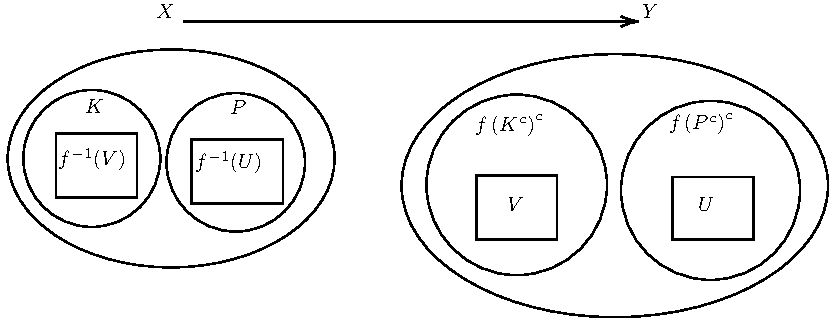
\includegraphics[scale=0.7]{T4.pdf}
        \end{figure}
    \end{proof}

    可以举出Hausdorff空间在商空间下不遗传的例子:考虑$\R/E$即可。这是一个开映射,因为任何开集都包含区间,
    而区间的像是整个$\R/E$。于是开集的像是全空间,是开映射。但是平庸拓扑显然不是$T_0$的。

    这说明,在商映射(开映射)下,$T_4$甚至不能保持$T_0$,于是Hausdorff更不能保证。

    一个值得思考的问题是,如果我们研究紧Hausdorff空间,那么是否会有一个比较好的结果来保证遗传呢?
    \begin{theorem}[Alexandroff定理]
        若$X$是紧Hausdorff空间,$E$是$X$上的等价关系,则下列条件等价:
        \begin{enumerate}
            \item $X/E$是紧Hausdorff空间。
            \item $E$是乘积空间$X \times X$的闭子集。
            \item 粘合映射$\rho:X \to X/E$是闭映射。
        \end{enumerate}
    \end{theorem}
    \begin{proof}
        如果$X/E$是紧Hausdorff空间,那么:
        $$
        E=\{(x,y)|q(x)=q(y)\}=\{(x,y)|q\circ p_1(x,y)=q\circ p_2(x,y)\}
        $$
        考虑$q,p_1,p_2$都是连续映射,并且$X/E$是Hausdorff空间,那么$E$是闭集。

        如果$E$是闭集,我们说明,对于任何$X$的闭集$A$,
        $\rho^{-1}(\rho(A))$也是闭集。即:
        $$
        \bigcup_{a\in A}[a]
        $$
        为闭集。考虑$x \notin \rho^{-1}(\rho(A))$,由于$\{x\}\times A$
        含于开集$(X\times X)\setminus E$,而$A$是紧子集,由管形引理知,存在$x$的
        开邻域$U$使得:
        $$
        (U \times A)\cap E=\emptyset
        $$
        于是$U \subset \rho^{-1}(\rho(A))^c$,这说明映射是闭映射。

        如果粘合映射是闭映射,那么首先作为紧空间的连续像,$X/E$是紧空间。
        其次,根据引理5.13,紧Hausdorff空间$T_4$,于是$X/E$是$T_4$的,从而满足Hausdorff
        性质。

    \end{proof}
    最后介绍一个推论,其余的代拓知识,请自行查看教材。
    \begin{corollary}
        设$X,Y$是紧Hausdorff空间;$E_x$是等价关系,并且是闭子集。$E_Y$类似。那么:
        $$
        (X \times Y)/(E_X\times E_Y)
        $$
        与
        $$
        (X/E_X)\times (Y/E_Y)
        $$
        同胚。
    \end{corollary}
    \begin{proof}
        留作复习的习题。
    \end{proof}
    \section{Urysohn引理和度量化定理}
    本章我们将讨论一个空间是否可度量化。这是一个很基本的问题,却有几个十分重要的定理。
    \subsection{Urysohn引理}
    \subsubsection{Urysohn引理}
    我们直截了当的给出这个引理:
    \begin{lemma}[Urysohn引理]{lem:Ury}
        设$X$是正规空间;$A$和$B$是$X$的不交闭集。则存在连续函数:
        $$
        f:X \to [0,1]
        $$
        满足:$\forall x \in A,f(x)=0;\forall x \in B,f(x)=1$。
    \end{lemma}
        
    我们先观察最特殊的情况——度量空间。设$A$,$B$是度量空间$(X,d)$中的
    不交非空闭集。定义$f$:
    $$
    f(x)=\frac{t_A(x)}{t_A(x)+t_B(x)}
    $$

    其中$t_A(x)=\inf_{y \in A}d(x,y)$。从而$f(A)=0,f(B)=1$。

    于是作为特殊的正规空间,我们给出了度量空间下该引理的证明。由于我们想研究“度量化”,那么
    不难想到,如果能证明该引理在一般情况下成立,那么在之后的研究中将会发挥极大的作用。

    再注意引理本身。它告诉我们,只要利用空间的内在性质就能给出该空间到其他空间的联系。这一点至关重要。
    \begin{lemma}
            设$X$是拓扑空间,$f:X \to \R$连续。则任给有理数$r$,$U_r=f^{-1}(r,\infty)$是$X$的开集。
            并且:
            $$
            f(x)=\sup\{r \in \Q|x \in U_r\}
            $$
    \end{lemma}
    \begin{proof}
        $x \in U_r$意味着$f(x)>r$。即$f(x)\geq \sup\{r \in \Q|x \in U_r\}$.

        若$f(x)>\sup\{r \in \Q|x \in U_r\}$,则有$q:f(x)>q>\sup\{r \in \Q|x \in U_r\}$。由于
        $f(x)>q$,则$x \in U_q$。然而$q>\sup\{r \in \Q|x \in U_r\}$,这矛盾!
    \end{proof}

    该引理说明,可以用开集族来描述连续函数。
    \begin{proof}[Urysohn引理]
        对于任意的$r \in \Q \cap[0,1]$,定义开集$U_r$使得:
        \begin{enumerate}
            \item $A \subset U_r \subset \overline{U_r} \subset B^c$.
            \item $r<s \Rightarrow U_r \subset \overline{U_r} \subset U_s \subset \overline{U_s}$
            \item $\bigcap_{r\in \Q}U_r =A$
            \item $\bigcup_{r \in \Q}U_r =B^c$
        \end{enumerate}
        构造这样的开集的原因在于:我们可以证明,满足上述性质的开集族$\{U_r\}$可以诱导
        一个连续函数,并且该函数满足$f(A)=0,f(B)=0$。

        首先我们证明满足这种性质的开集是可以构造的:
    
        我们把$[0,1]$中所有有理数排列:$r_0,r_1,\dots$,并保证
        $r_0=0,r_1=1$.我们用归纳法来得到满足这样条件的开集:
        
        对于$n=1$,从正规我们有:存在开集$V:A \subset V \subset \overline{V}
        \subset X\setminus A$.令$U_{r_0}=V,U_{r_1}=X\setminus A$。我们就得到了满足
        要求的集合。

        假设我们现在已经构造了$n+1$个集合满足上述四个条件。
        现在要构造$V_{r_{n+1}}$。考虑我们
        之前所要求的集合的性质,我们考虑:
        $$
        r_L=\max\{r_i|r_i<r_{n+1},i \leq n\},\qquad r_R=\min\{r_i|r_i>r_{n+1},i\leq n\}
        $$
        注意这等于是把$r_{n+1}$按照大小顺序嵌入了原来的$n+1$个数中。
        现在$U_{r_R}$和$U_{r_L}$分别在$U_{r_{n+1}}$的右,左。
        考虑到$\overline{U_{r_L}}\subset U_{r_R}$,于是再次根据正规:
        $$
        \exists O, \overline{U_{r_L}}\subset O \subset \overline{O}\subset U_{r_R}
        $$
        从而令$U_{r_{n+1}}=O$即可。

        通过验证,新增加的集合$O$并不违背1,3,4。于是我们证明了,我们可以按照这种方法构造出可数个集合列。存在性得证。

        接下来我们说明这样的集族$\{U_r\}$决定的函数:
        $$
        f:X \to\R,\qquad f(x)=\sup\{r \in \Q|x \in U_r\}
        $$
        是连续的即可。因为其本身已经满足:$f(A)=0,f(B)=0$。

        我们只用验证$\R$上基的原像是开集,即:
        $$
        f^{-1}(a,+\infty)=\{x \in X|\exists r\in \Q,f(x)>r>a\}=\bigcup\{U_r|r>a\}
        $$
        是开集。
        
        和:
        $$
        f^{-1}(-\infty,a)=\bigcup\{X\setminus \overline{U_r}|r\in \Q,r<a\}
        $$
        原因是因为,一旦$f(x)<a$,那么$f(x)<r<s<a$。于是$x \in U_s^c$。注意到$r<s$,于是$\overline{U_r}^c \supset U_s^c$。于是
        $x \in \overline{U_r}^c$。
        
        另一方面,如果$x \in \overline{U_s}^c$,
        那么就有$f(x)\leq s$(若不然,则$f(x)>s$,于是$x \in U_s$。)于是右边也能推导左边。
    \end{proof}
    \subsubsection{Hahn-Tong插入定理}
    \begin{definition}
        设$X$是拓扑空间,
        称$f:X \to \R$下半连续,
        若任给$t\in \R$,$\{x \in X|f(x)\leq t\}$是$X$闭子集。
        称$f:X \to \R$上半连续,
        若任给$t\in \R$,$\{x \in X|f(x)\geq t\}$是$X$闭子集。
    \end{definition}
        显然,如果只关注右拓扑,那么上半连续意味着右拓扑连续。只关注左拓扑,
        那么下半连续意味着左拓扑连续。
        \begin{proposition}
            \begin{enumerate}
                \item 连续当且仅当上半连续+下半连续。
                \item 集合$A$的特征函数上半连续当且仅当为闭集;下半连续当且仅当为开集。
                \item $f$和$g$都是下(上)半连续函数,则$f \wedge g$与$f\vee g$都是下(上)
                半连续函数。
            \end{enumerate}
        \end{proposition}
        证明留作复习习题。

    \begin{theorem}[Hahn-Tong插入定理]
        设$X$是正规空间,$h:X \to \R$下半连续,$g: X \to \R$上半连续。并且$g(x)\leq h(x)$。则存在连续函数:
        $$
        f:X \to \R, \qquad g \leq f\leq h
        $$
    \end{theorem} 
    我们注意到,如果$F$,$P$是$X$的不相交闭集,那么$\chi_F,\chi_{P^c}$一个是上半连续的,一个是下半连续的。
    并且$\chi_F \leq \chi_{P^c}$。那么根据Hahn-Tong插入定理,就有连续函数$f$:
    $$
    \chi_F \leq f \leq \chi_{P^c}
    $$
    注意到
    $x \in F$,则$f(x)=1$;$x\in P$,则$f(x)=0$。
    于是Hahn-Tong插入定理可以推导Urysohn定理。

    上述这一事实也提供了证明Hahn-Tong插入定理的思路。
    \begin{proof}
        
    \end{proof}
    \begin{theorem}[Tietze扩张定理]
        设$X$是正规空间,$M$是$X$中的闭集,$f:M \to \R$是
        连续函数。则存在连续函数$f^*: X \to \R$使得:
        $$
        f^*|_M=f
        $$
        
    \end{theorem}
    \begin{proof}
        首先考虑$f$有界的情况。

        此时,考虑$g=f\chi_M$。$g$是上半连续的,因为:
        $$
        \{g \geq t\}=\{f \geq t\} \cap M
        $$
        是闭集。

        同时,$h=f,x \in M;=1,x \notin M$.此时$h$下半连续。
        运用Hahn-Tong插入定理即可得到答案。

        如果$f$不是有界的,用$\R \to (-1,1)$的一个同胚来考虑问题:
        $$
        \tilde{f}= \varphi \circ f 
        $$
        则
    \end{proof}
    \subsection{Urysohn度量化定理}
    \begin{theorem}[Urysohn度量化定理]
        第二可数的$T_4$空间可度量化。
    \end{theorem}
    \begin{proof}
        设$\{U_n\}$是空间的可数基。
    \end{proof}
    \end{document}

